Zu Beginn dieses Unterkapitels soll die bereits erwähnte \acf{pwa} erklärt werden. Anschließend folgen die verwendeten Frameworks für die Entwicklung der \ac{pwa}. Ein Überblick über diese ist essenziell für das Verständnis von Kapitel \ref{chap:implementierung}, in welchem die Implementierungsschritte betrachtet werden.

Eine Progressive Web App ist ein nächster Schritt nach der Dynamisierung statischer HTML-Seiten durch JavaScript und Frontendframeworks. Der Software Entwickler und Autor Majid Hajian charakterisiert \ac{pwa}s mit acht Eigenschaften. Die wichtigsten dieser Charakteristika werden im Folgenden zusammenfassend erläutert:


\begin{description}
  \item [Installierbarkeit]
	  Der*die Nutzer*in einer Webanwendung kann diese lokal auf seinem Gerät installieren. Sie kann anschließend, wie eine native App, vom Startbildschirm gestartet werden. Um die Webanwendung zu Nutzen muss ein*e Nutzer*in keinen Zwischenschritt mehr über den Browser tätigen.
  
  \item [Ähnlichkeit mit einer nativ implementierten App]  
 	 Klassischerweise werden Android-Apps in Java und iOS Apps in Swift programmiert. Die \ac{pwa} soll, wie eine native App, auf die Hardware des Mobilgeräts zugreifen können (beispielsweise die Nutzung Bluetooth-Chips). Außerdem unterscheidet sich das User Interface der \ac{pwa} nicht maßgeblich von der nativen App. 
  
  \item [Offline-Verwendung] 
  	Die \ac{pwa} soll unabhängig von Netzwerkverbindung funktionieren. Sie ist nach dem "offline-first-design" konzipiert. Die Google-Chrome Dokumentation für Cloud-Entwickler beschreibt Offline First Apps als Webanwendung, deren Dateien (JavaScript, HTML, CSS etc.) bereits heruntergeladen sind. Daten werden temporär über eine Browser-Schnittstelle gespeichert und bei Bedarf synchronisiert. Außerdem kann die Anwendung auf eine unterbrochene Netzwerkverbindungen reagieren \cite{GoogleOfflineApps}. Die \ac{pwa} ist demnach eine Webanwendung, die sowohl online, als auch offline nutzbar ist.

  \item [Mobiloptimiert]  
  	Die \ac{pwa} ist für die (meist leistungsschwache) Mobilhardware konzipiert und funktioniert hierauf ohne Performanzprobleme. Hajian legt besonders auf das schnelle Laden beim Start der Anwendung wert.
  	
  \item [Informierung des Nutzers] 
  	Wie native Apps, kann die \ac{pwa} den Nutzer über Push-Nachrichten informieren oder zu Interaktion auffordern.
\end{description}

\cite[S. 1f.]{Hajian2019}
Diese Charakteristiken decken sich mit der Beschreibung durch die Entwickler-Dokumentation der \ac{pwa} von Google. Im Vergleich zu Hijian ist diese etwas spezifischer und erwähnt beispielsweise die Kontrolle des Anwendungscaches durch einen JavaScript Service Worker (siehe Kapitel \ref{chap:service_worker}), um die Abhängigkeit von einer Netzwerkverbindung aufzuheben.
\cite{GooglePWAOverview}

\subsection{Installation einer Progressive Web App}

Diese Arbeit betrachtet die \ac{pwa}, da sie (wie eine native Anwendung) lokal auf einem Gerät installiert werden kann. Es ist dafür kein zentraler Shop nötig: die Installation wird über den Browser gestartet.

\begin{figure}[h]
        \centering
        
\includegraphics[scale=0.2]{img/a2hs-infobar-cropped.png}
        \caption{Browserdialog zur Installation einer \ac{pwa} \cite{PWAAddToHomeScreenPrompt}}
        \label{fig:pwainstallationprompt}
\end{figure}

Die Aufforderung zur Installation einer \ac{pwa} kann entweder über den Browser (siehe Abbildung \ref{fig:pwainstallationprompt}) erfolgen oder über ein Element der Website, dass ein Event erzeugt, wie beispielsweise ein Button oder ein Dialog. 

Zwar bezeichnen Browser die Installation meist nur als \texttt{Zum Startbildschirm hinzufügen} tatsächlich generiert der Browser aber dann eine WebAPK, welche auf dem Gerät installiert wird. Auf Desktopgeräte startet die \ac{pwa} in einem eignen stark verschlankten Browserfenster ohne Suchleiste und Bedienelemente. \cite{GooglePWAInstallation}


\subsection{Manifest Datei für die Konfiguration der \ac{pwa}}

Um die \ac{pwa} auf einem Gerät installieren zu können, muss es eine \textit{web-app-manifest} Datei zur Verfügung gestellt werden. Diese ist ein \ac{json} file, welche als Konfigurationsdatei der installierten Anwendung dient. \cite{GooglePWAManifest}

\begin{listing}[H]
    \inputminted{json}{sourcecode/manifest_sample.json}
    \caption{Manifestdatei einer \ac{pwa}}
      \label{sourcecode:manifest_sample}
\end{listing}

Quellcode-Abschnitt \ref{sourcecode:manifest_sample} zeigt den Inhalt einer Manifest-Datei. Neben diversen Icons (Zeile 4-15) werden auch \textit{Name} (Zeile 3), \textit{Farbschema} (Zeile 20) und \textit{Anzeigeeinstellungen} (Zeile 18) festgelegt.
Die Manifest-Datei wird im HTML der Webanwendung eingebunden, siehe Quellcode-Abschnitt \ref{sourcecode:manifest_include}. 

Es ist die Einfachheit dieses Prozesses hervorzuheben: Das Hinzufügen einer (wenige Zeilen langer) \ac{json}-Datei macht die gesamte Webanwendung installierbar. Es wird kein App-Store, manueller Dateidownload oder Installer benötigt. 

\begin{listing}[H]
    \inputminted{xml}{sourcecode/include_manifest.html}
    \caption{Einbinden der Manifestdatei}
      \label{sourcecode:manifest_include}
              %https://developers.google.com/web/fundamentals/web-app-manifest?hl=en
\end{listing}

%\begin{figure}[h]
%        \centering
%%        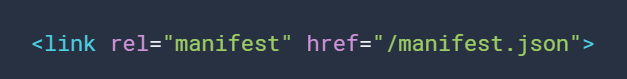
\includegraphics[scale=0.7]{img/include_manifest.png}
 %%       \caption{Einfache Einbindung des Manifests}
  %      \label{sourcecode:manifest_include}
        %https://developers.google.com/web/fundamentals/web-app-manifest?hl=en
%\end{figure}


\subsection{Service Worker für Offline-Funktionalität und Benachrichtigungen}
\label{chap:service_worker}

Damit die \ac{pwa} trotz fehlender Netzwerkverbindung funktioniert wird ein besonderer Mechanismus benötigt: der Service Worker. Mit ihm können Abhängigkeiten der App lokal gecached werden, so dass die Anwendung auch bei schlechter oder gar fehlender Netzwerkverbindung funktioniert. \cite[S. 7]{BeginningPWA}

Ein Service Worker ist ein von der UI separiert laufendes Hintergrundskript der Webanwendung, siehe Abbildung \ref{fig:serviceWorker}. Er wird genutzt um Bilder, Skripts, Styles oder ganze Seiten zu cachen. Bei bestehender Netzwerkverbindung führt er nötige Synchronisierungen durch. Nicht zuletzt ist er auch für das senden von Push-Notifications zuständig. \cite[S. 24]{BeginningPWA}

\begin{figure}[h]
        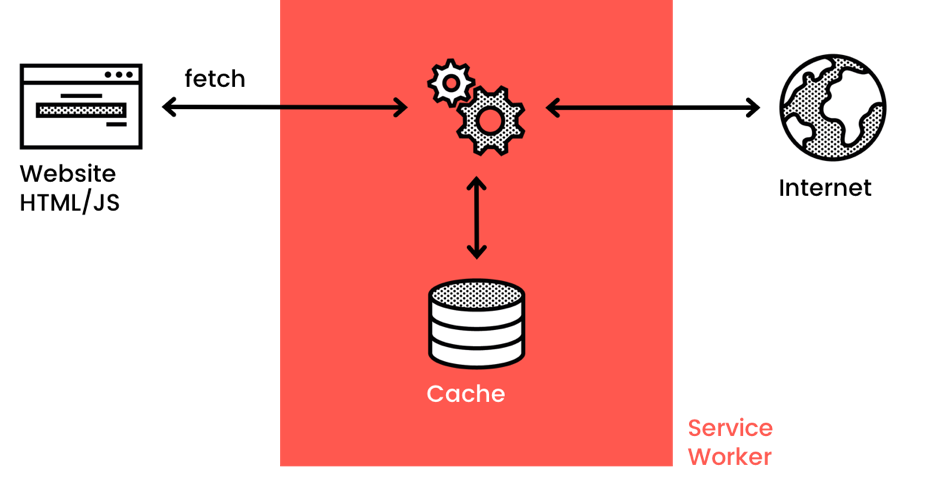
\includegraphics[width=\linewidth]{img/ServiceWorker-8a0968f1b295f1ff.png}
        \centering
        \caption{Konzept des Service Workers \cite{ServiceWorkerDiagramm}}
        \label{fig:serviceWorker}
\end{figure}


Alle verbreiteten Desktopbrowser wie Chrome, Firefox, Opera, Edge und mittlerweile auch Safari unterstützen das Service Worker Konzept. Der Mobile Chromebrowser unter Android unterstützt Service Worker bereits voll, während Safari unter iOS noch an diesem Feature arbeitet. \cite[S. 9]{BeginningPWA}


\subsection{Plattformen von eine \ac{pwa} aktuell unterstützen}
Das Projekt \textit{CanIUse} aggregiert Daten zu Webstandards des w3 Konsortiums und Browserdokumentationen. Es wird als Quelle für die Unterstützung von Features durch aktuelle Browser herangezogen.

Apples mobiler Browser Safari unterstützt eines der wichtigsten Features der \ac{pwa} noch nicht vollständig: das Web App Manifest. Allerdings wird der Service Worker vollständig unterstützt \cite{CanIUseWebManifest}. Wann und ob Safari die Unterstützung für das Manifest implementiert ist unklar und bleibt abzuwarten. Die aktuelle Teilunterstützung zeigt jedoch, dass sich Apple nicht grundsätzlich gegen die \ac{pwa} weigert.

 %Die Versionen zeigen aber eine stetig voranschreitende Integration der, erweitert den Funktionsumfang in den neusten Versionen von iOS. 

% https://medium.com/@firt/progressive-web-apps-on-ios-are-here-d00430dee3a7



% Source: https://developers.google.com/web/progressive-web-apps/desktop
Die Nutzung von \ac{pwa}s ist nicht ausschließlich auf Smartphones begrenzt. Wie normale Desktopprogramme werden Desktop \ac{pwa}s in einem eigenen Fenster gestartet. 
Der Unterschied zwischen den Bedienelementen nativer Desktopanwendungen und Desktop \ac{pwa}s ist ausschließlich farblicher Natur. Stark vereinfacht beschrieben, sind Desktop \ac{pwa}s Browserfenster ohne Tabs und Adressleiste. Durch die Nutzung von Service Workern, welche die Webanwendung cachen, sind auch Desktop \ac{pwa}s nicht an eine Netzwerkverbindung gebunden.

Grundsätzlich können Desktop \ac{pwa}s auf jedem Betriebssystem installiert werden, auf dem Google Chrome (Version größer 73) installiert werden kann: Windows, Mac, Linux und Chrome OS.
\cite{GooglePWADesktop}



\subsection{Grundlage der Webanwendung: JavaScript Laufzeitumgebung Node.js}

%NodeJSWebsiteAbout
\textit{Node.js} ist eine open-source JavaScript Laufzeitumgebung für die Entwicklung skalierbarer Webanwendungen 
\cite{NodeJSWebsiteAbout}.
Selbst baut Node.js auf der \textit{V8-Engine} auf, einer Laufzeitumgebung, die auch von Google Chrome genutzt wird 
%NodeJSRecepies
\cite[S. 1]{NodeJSRecepies}.
% PracitalNodeJS
Wegen zeitsparenden Features, wie automatischem Typecasting oder der Tatsache, dass Node.js alle Daten als Objekt behandelt, erfreut sich Node.js großer Beliebtheit 
\cite[S. 12]{PracitalNodeJS}.
Die Kombination mit dem \textit{Package Manager npm} ermöglicht die einfache Installation und Nutzung von Modulen, um die Funktionalität der Plattform zu erweitern. 
\cite[S. 9]{NodeJSRecepies}.


\subsection{Frontend-Framwork Angular für die Entwicklung von Webanwendungen}

Angular ist ein open-source TypeScript basiertes Framework zur Entwicklung von Webanwendungen, welches Node.js nutzt.


%https://octoverse.github.com/projects
Mit über Achttausend Mitwirkenden Entwicklern (Angular CLI) beziehungsweise über Siebentausend Mitwirkender (Angular Framework) belegt das Angular Command Line Interface und das Angular Framework die Plätze 4 und 6 der größten Projekte auf Github. 
% https://octoverse.github.com/projects
\cite{OctoverseGitHubStatistics}

Das Framework arbeitet auf Basis von Komponenten. Ein Eingabefeld, Seite oder eine Liste werden in Angular als solche Komponenten separat betrachtet. Auch in der Dateistruktur werden Komponenten stark getrennt. Jede Komponente besitzt beispielsweise ein eigenes CSS (oder SCSS) und HTML-File. Eine Komponente für eine Seite kann so auch eine oder sogar mehrere Listenkomponenten einbinden. Durch die Wiederverwendung von Code-Fragmenten in Komponenten wird der Programmcode sehr übersichtlich und strukturiert.

\begin{figure}[h]
        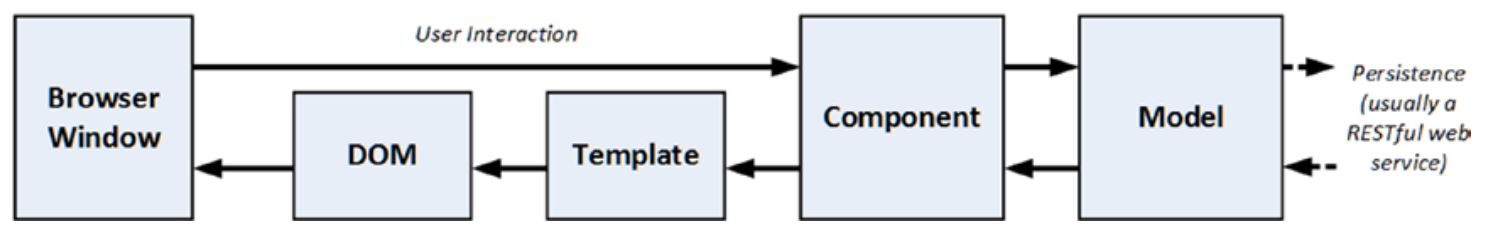
\includegraphics[width=\linewidth]{img/Angular_MVC.JPG}
        \centering
        \caption{MVC Konzept von Angular \cite[S. 35, Abbildung 3-4]{ProAngular}}
        \label{fig:angularmvc}
\end{figure}

Eine Angular Anwendung ist in drei Einheiten gegliedert:\\

\textbf{Model}\\ 
Enthält Logik für die Verwaltung von Daten, beispielsweise das Erstellen, Speichern oder Modifizieren. Dies kann über die Kommunikation mit einem Webserver via REST-API erfolgen. Das Model enthält keine Logik, um mit dem Nutzer zu interagieren.\\

\textbf{Component}\\
Enthält Logik für das Aktualisieren der Daten im Model aufgrund Nutzerinteraktion. \\

\textbf{Template}\\ 
Enthält Logik und Markup, um dem Nutzer Daten anzeigen zu können.

\cite{ProAngular}